\documentclass[11pt,a4paper,]{article}
\usepackage{lmodern}

\usepackage{amssymb,amsmath}
\usepackage{ifxetex,ifluatex}
\usepackage{fixltx2e} % provides \textsubscript
\ifnum 0\ifxetex 1\fi\ifluatex 1\fi=0 % if pdftex
  \usepackage[T1]{fontenc}
  \usepackage[utf8]{inputenc}
\else % if luatex or xelatex
  \usepackage{unicode-math}
  \defaultfontfeatures{Ligatures=TeX,Scale=MatchLowercase}
\fi
% use upquote if available, for straight quotes in verbatim environments
\IfFileExists{upquote.sty}{\usepackage{upquote}}{}
% use microtype if available
\IfFileExists{microtype.sty}{%
\usepackage[]{microtype}
\UseMicrotypeSet[protrusion]{basicmath} % disable protrusion for tt fonts
}{}
\PassOptionsToPackage{hyphens}{url} % url is loaded by hyperref
\usepackage[unicode=true]{hyperref}
\hypersetup{
            pdftitle={Urbanization, energy consumption, and CO2 emissions with different income level countries},
            pdfborder={0 0 0},
            breaklinks=true}
\urlstyle{same}  % don't use monospace font for urls
\usepackage{geometry}
\geometry{a4paper, centering, text={16cm,24cm}}
\usepackage[style=authoryear-comp,]{biblatex}
\addbibresource{references.bib}
\usepackage{longtable,booktabs}
% Fix footnotes in tables (requires footnote package)
\IfFileExists{footnote.sty}{\usepackage{footnote}\makesavenoteenv{long table}}{}
\usepackage{graphicx,grffile}
\makeatletter
\def\maxwidth{\ifdim\Gin@nat@width>\linewidth\linewidth\else\Gin@nat@width\fi}
\def\maxheight{\ifdim\Gin@nat@height>\textheight\textheight\else\Gin@nat@height\fi}
\makeatother
% Scale images if necessary, so that they will not overflow the page
% margins by default, and it is still possible to overwrite the defaults
% using explicit options in \includegraphics[width, height, ...]{}
\setkeys{Gin}{width=\maxwidth,height=\maxheight,keepaspectratio}
\IfFileExists{parskip.sty}{%
\usepackage{parskip}
}{% else
\setlength{\parindent}{0pt}
\setlength{\parskip}{6pt plus 2pt minus 1pt}
}
\setlength{\emergencystretch}{3em}  % prevent overfull lines
\providecommand{\tightlist}{%
  \setlength{\itemsep}{0pt}\setlength{\parskip}{0pt}}
\setcounter{secnumdepth}{5}

% set default figure placement to htbp
\makeatletter
\def\fps@figure{htbp}
\makeatother

% NEW:set default table placement to htbp
\makeatletter
\def\fps@table{htbp}
\makeatother

\title{Urbanization, energy consumption, and CO2 emissions with different income level countries}

%% MONASH STUFF

%% CAPTIONS
\RequirePackage{caption}
\DeclareCaptionStyle{italic}[justification=centering]
 {labelfont={bf},textfont={it},labelsep=colon}
\captionsetup[figure]{style=italic,format=hang,singlelinecheck=true}
\captionsetup[table]{style=italic,format=hang,singlelinecheck=true}


%% FONT
\RequirePackage{bera}
\RequirePackage[charter,expert,sfscaled]{mathdesign}
\RequirePackage{fontawesome}

%% HEADERS AND FOOTERS
\RequirePackage{fancyhdr}
\pagestyle{fancy}
\rfoot{\Large\sffamily\raisebox{-0.1cm}{\textbf{\thepage}}}
\makeatletter
\lhead{\textsf{\expandafter{\@title}}}
\makeatother
\rhead{}
\cfoot{}
\setlength{\headheight}{15pt}
\renewcommand{\headrulewidth}{0.4pt}
\renewcommand{\footrulewidth}{0.4pt}
\fancypagestyle{plain}{%
\fancyhf{} % clear all header and footer fields
\fancyfoot[C]{\sffamily\thepage} % except the center
\renewcommand{\headrulewidth}{0pt}
\renewcommand{\footrulewidth}{0pt}}

%% MATHS
\RequirePackage{bm,amsmath}
\allowdisplaybreaks

%% GRAPHICS
\RequirePackage{graphicx}
\setcounter{topnumber}{2}
\setcounter{bottomnumber}{2}
\setcounter{totalnumber}{4}
\renewcommand{\topfraction}{0.85}
\renewcommand{\bottomfraction}{0.85}
\renewcommand{\textfraction}{0.15}
\renewcommand{\floatpagefraction}{0.8}


%\RequirePackage[section]{placeins}

%% SECTION TITLES


%% SECTION TITLES (NEW: Changing sections and subsections color)
\RequirePackage[compact,sf,bf]{titlesec}
\titleformat*{\section}{\Large\sf\bfseries\color[rgb]{0.8, 0.7, 0.1 }}
\titleformat*{\subsection}{\large\sf\bfseries\color[rgb]{0.8, 0.7, 0.1 }}
\titleformat*{\subsubsection}{\sf\bfseries\color[rgb]{0.8, 0.7, 0.1 }}
\titlespacing{\section}{0pt}{2ex}{.5ex}
\titlespacing{\subsection}{0pt}{1.5ex}{0ex}
\titlespacing{\subsubsection}{0pt}{.5ex}{0ex}


%% TITLE PAGE
\def\Date{\number\day}
\def\Month{\ifcase\month\or
 January\or February\or March\or April\or May\or June\or
 July\or August\or September\or October\or November\or December\fi}
\def\Year{\number\year}

%% LINE AND PAGE BREAKING
\sloppy
\clubpenalty = 10000
\widowpenalty = 10000
\brokenpenalty = 10000
\RequirePackage{microtype}

%% PARAGRAPH BREAKS
\setlength{\parskip}{1.4ex}
\setlength{\parindent}{0em}

%% HYPERLINKS
\RequirePackage{xcolor} % Needed for links
\definecolor{darkblue}{rgb}{0,0,.6}
\RequirePackage{url}

\makeatletter
\@ifpackageloaded{hyperref}{}{\RequirePackage{hyperref}}
\makeatother
\hypersetup{
     citecolor=0 0 0,
     breaklinks=true,
     bookmarksopen=true,
     bookmarksnumbered=true,
     linkcolor=darkblue,
     urlcolor=blue,
     citecolor=darkblue,
     colorlinks=true}

\usepackage[showonlyrefs]{mathtools}
\usepackage[no-weekday]{eukdate}

%% BIBLIOGRAPHY

\makeatletter
\@ifpackageloaded{biblatex}{}{\usepackage[style=authoryear-comp, backend=biber, natbib=true]{biblatex}}
\makeatother
\ExecuteBibliographyOptions{bibencoding=utf8,minnames=1,maxnames=3, maxbibnames=99,dashed=false,terseinits=true,giveninits=true,uniquename=false,uniquelist=false,doi=false, isbn=false,url=true,sortcites=false}

\DeclareFieldFormat{url}{\texttt{\url{#1}}}
\DeclareFieldFormat[article]{pages}{#1}
\DeclareFieldFormat[inproceedings]{pages}{\lowercase{pp.}#1}
\DeclareFieldFormat[incollection]{pages}{\lowercase{pp.}#1}
\DeclareFieldFormat[article]{volume}{\mkbibbold{#1}}
\DeclareFieldFormat[article]{number}{\mkbibparens{#1}}
\DeclareFieldFormat[article]{title}{\MakeCapital{#1}}
\DeclareFieldFormat[article]{url}{}
%\DeclareFieldFormat[book]{url}{}
%\DeclareFieldFormat[inbook]{url}{}
%\DeclareFieldFormat[incollection]{url}{}
%\DeclareFieldFormat[inproceedings]{url}{}
\DeclareFieldFormat[inproceedings]{title}{#1}
\DeclareFieldFormat{shorthandwidth}{#1}
%\DeclareFieldFormat{extrayear}{}
% No dot before number of articles
\usepackage{xpatch}
\xpatchbibmacro{volume+number+eid}{\setunit*{\adddot}}{}{}{}
% Remove In: for an article.
\renewbibmacro{in:}{%
  \ifentrytype{article}{}{%
  \printtext{\bibstring{in}\intitlepunct}}}

\AtEveryBibitem{\clearfield{month}}
\AtEveryCitekey{\clearfield{month}}

\makeatletter
\DeclareDelimFormat[cbx@textcite]{nameyeardelim}{\addspace}
\makeatother

\author{\sf\Large\textbf{ Di Cui}\\ {\sf\large Master of Business Analytics\\[0.5cm]} \sf\Large\textbf{ Guanru Chen}\\ {\sf\large Master of Business Analytics\\[0.5cm]} \sf\Large\textbf{ Yunzhi Chen}\\ {\sf\large Master of Business Analytics\\[0.5cm]}}

\date{\sf\Date~\Month~\Year}
\makeatletter
\lfoot{\sf Cui, Chen, Chen: \@date}
\makeatother


%%%% PAGE STYLE FOR FRONT PAGE OF REPORTS

\makeatletter
\def\organization#1{\gdef\@organization{#1}}
\def\telephone#1{\gdef\@telephone{#1}}
\def\email#1{\gdef\@email{#1}}
\makeatother
  \organization{World Bank}

  \def\name{TGIF \newline Di Cui \&\newline Guanru Chen \&\newline Yunzhi Chen}

  \telephone{(03) 9905 2478}

  \email{questions@company.com}                 %NEW: New email addresss

\def\webaddress{\url{http://company.com/stats/consulting/}} %NEW: URl
\def\abn{12 377 614 630}                                    % NEW: ABN
\def\logo{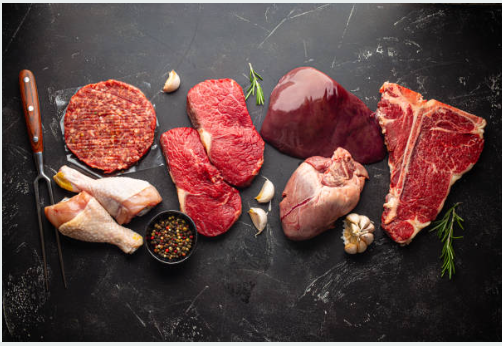
\includegraphics[width=6cm]{Figures/logo}}  %NEW: Changing logo
\def\extraspace{\vspace*{1.6cm}}
\makeatletter
\def\contactdetails{\faicon{phone} & \@telephone \\
                    \faicon{envelope} & \@email}
\makeatother

%%%% FRONT PAGE OF REPORTS

\def\reporttype{Report for}

\long\def\front#1#2#3{
\newpage
\begin{singlespacing}
\thispagestyle{empty}
\vspace*{-1.4cm}
\hspace*{-1.4cm}
\hbox to 16cm{
  \hbox to 6.5cm{\vbox to 14cm{\vbox to 25cm{
    \logo
    \vfill
    \parbox{6.3cm}{\raggedright
      \sf\color[rgb]{0.8, 0.7, 0.1 }    % NEW color 
      {\large\textbf{\name}}\par
      \vspace{.7cm}
      \tabcolsep=0.12cm\sf\small
      \begin{tabular}{@{}ll@{}}\contactdetails
      \end{tabular}
      \vspace*{0.3cm}\par
      ABN: \abn\par
    }
  }\vss}\hss}
  \hspace*{0.2cm}
  \hbox to 1cm{\vbox to 14cm{\rule{4pt}{26.8cm}\vss}\hss\hfill}  %NEW: Thicker line
  \hbox to 10cm{\vbox to 14cm{\vbox to 25cm{   
      \vspace*{3cm}\sf\raggedright
      \parbox{11cm}{\sf\raggedright\baselineskip=1.2cm
         \fontsize{24.88}{30}\color[rgb]{0, 0.29, 0.55}\sf\textbf{#1}}   % NEW: title color blue
      \par
      \vfill
      \large
      \vbox{\parskip=0.8cm #2}\par
      \vspace*{2cm}\par
      \reporttype\\[0.3cm]
      \hbox{#3}%\\[2cm]\
      \vspace*{1cm}
      {\large\sf\textbf{\Date~\Month~\Year}}
   }\vss}
  }}
\end{singlespacing}
\newpage
}

\makeatletter
\def\titlepage{\front{\expandafter{\@title}}{\@author}{\@organization}}
\makeatother

\usepackage{setspace}
\setstretch{1.5}

%% Any special functions or other packages can be loaded here.
\usepackage{booktabs}
\usepackage{longtable}
\usepackage{array}
\usepackage{multirow}
\usepackage{wrapfig}
\usepackage{float}
\usepackage{colortbl}
\usepackage{pdflscape}
\usepackage{tabu}
\usepackage{threeparttable}
\usepackage{threeparttablex}
\usepackage[normalem]{ulem}
\usepackage{makecell}
\usepackage{xcolor}


\begin{document}
\titlepage

\hypertarget{data-set-introduction}{%
\section{Data set introduction}\label{data-set-introduction}}

At the World Bank, the Development Data Group coordinates statistical and data work and maintains a number of macro, financial and sector databases. The data set that we used was obtained from the World Bank database. This report explores the variation in data for six countries in different income groups by focusing on three variables of the data set: CO2 emissions (metric tons per capita), urban population and energy use (kg of oil equivalent per capita).

The CO2 emissions refers to annual anthropogenic emissions from data on fossil fuel consumption and world cement manufacturing.

Urban population refers to people living in urban areas as defined by national statistical offices.

Total energy use includes energy usage from combustible renewable and waste - solid biomass and animal products, gas and liquid from biomass, and industrial and municipal waste.

More information available \href{https://data.worldbank.org/}{here}.

\hypertarget{research-questions}{%
\section{Research questions}\label{research-questions}}

\begin{itemize}
\item
  For China and India, which country has more CO2 emissions per capita during 1960 to 2020?
\item
  How did the CO2 emissions per capita of China and India develop from 1960 to 2020?
\item
  How's the development of urbanization of the two selected countries of two types of income group:

  \begin{enumerate}
  \def\labelenumi{\arabic{enumi}.}
  \tightlist
  \item
    Ethiopia: Low income.
  \item
    Italy: High income
  \end{enumerate}
\item
  Would the situation be similar with the other income group countries.

  Is the situation similar with the status of observation from last question.
\item
  Overall energy use kg of oil\_equivalent per capita in Belgium and Turkey from 1960 to 2015.
\item
  The trend in energy use kg of oil\_equivalent per capita of Belgium and Turkey from 1960 to 2015.
\end{itemize}

\clearpage

\hypertarget{exploratory-data-analysis}{%
\section{Exploratory data analysis}\label{exploratory-data-analysis}}

\section*{Country China and India}

\subsection*{Analysis}

\textbf{Q1:}

\begin{table}

\caption{\label{tab:co2table}The mean and median of CO2 emissions(metric tones per capita) in China and India }
\centering
\begin{tabular}[t]{l|r|r}
\hline
Country\_Name & mean & median\\
\hline
China & 2.5792506 & 2.0384107\\
\hline
India & 0.7221454 & 0.5959397\\
\hline
\end{tabular}
\end{table}

In table\ref{tab:co2table}, we observe the mean and median of CO2 emissions per capita in China are all higher than the mean and median in India. The mean and median in China are all over 2 metric tons. However, the mean and median in India are all under 1 metric tons.

\textbf{Q2:}

\begin{figure}
\centering
\includegraphics{report_files/figure-latex/co2trend-1.pdf}
\caption{\label{fig:co2trend}The CO2 emissions(metric tones per capita) in China and India}
\end{figure}

Figure\ref{fig:co2trend} shows the uptrend development of CO2 emissions per capita in China and India. In China, the number of CO2 emissions per capita decreased after 1960, but the number has increased from 1970 and raised sharply from 2000, and the number has arrived at around 6.5 metric tons in 2010. In India, although the number increased all the time, the number was always under 2 metric tons.

\clearpage

\section*{Country Ethiopia and Italy}

\subsection*{Exploratory data analysis}

\begin{table}

\caption{\label{tab:tab2}Urban population per year of Ethiopia and Italy from 1999-2018}
\centering
\begin{tabular}[t]{rrr}
\toprule
Year & Ethiopia & Italy\\
\midrule
1999 & 9363839 & 38226137\\
2000 & 9761536 & 38277624\\
2001 & 10174157 & 38333314\\
2002 & 10604081 & 38447500\\
2003 & 11049316 & 38686985\\
\addlinespace
2004 & 11510093 & 39006818\\
2005 & 11986371 & 39267369\\
2006 & 12478999 & 39454178\\
2007 & 13001478 & 39722857\\
2008 & 13689470 & 40056298\\
\addlinespace
2009 & 14413055 & 40308358\\
2010 & 15178365 & 40502481\\
2011 & 15986316 & 40641670\\
2012 & 16839218 & 40894259\\
2013 & 17717910 & 41548775\\
\addlinespace
2014 & 18635946 & 42109853\\
2015 & 19590313 & 42247229\\
2016 & 20581872 & 42351339\\
2017 & 21609845 & 42462869\\
2018 & 22678295 & 42566587\\
\bottomrule
\end{tabular}
\end{table}

Because the data is across over 40 years, which is a bit longer to present. So in Table \ref{tab:tab2} we extract the urban population of two countries since 1999. And noticeably, the urban population of Ethiopia is lower than Italy throughout the whole period.

\begin{figure}
\centering
\includegraphics{report_files/figure-latex/fig2-1.pdf}
\caption{\label{fig:fig2}Comparison of the urbanization development}
\end{figure}

In figure \ref{fig:fig2} we observe the level of urbanization in Ethiopia is still strong, but on the other hand, Italy is quite stable. And we observe the similar trend in the plot of income group.

Based on this finding, we may conclude that the level of urbanization of the country may be significantly affected by its development of economic and its state income.

\clearpage

\section*{Country Belgium and Turkey}

\subsection*{Analysis}

\textbf{The total energy use of Belgium and Turkey}

From 1960 to 2015, the total energy use of Belgium is 258677.63 kg of oil\_equivalent per capita, while it is 51666.23 kg in Turkey. See Table \ref{tab:energyuse-Tot}.

\begin{table}

\caption{\label{tab:energyuse-Tot}Total energy use of Belgium and Turkey}
\centering
\begin{tabular}[t]{l|r}
\hline
Country\_Name & Total\_energy\_use\\
\hline
Belgium & 258677.63\\
\hline
Turkey & 51666.23\\
\hline
\end{tabular}
\end{table}

\textbf{The trend}

Figure \ref{fig:trend} shows the trend of the energy use kg of oil\_equivalent per capita in Belgium and Turkey. In general, energy use kg of oil\_equivalent per capita in both countries shows an upward trend over the 55-year period, but Belgium's energy use is much higher than Turkey's. Belgium shows a fluctuating upward trend, with a larger increase than Turkey, while Turkey shows a steady upward trend.

\begin{figure}
\centering
\includegraphics{report_files/figure-latex/trend-1.pdf}
\caption{\label{fig:trend}Energy use of Belgium and Turkey}
\end{figure}

\hypertarget{visualization-of-urbanization-energy-consumption-and-co2-emissions-with-different-income-level-countries}{%
\section{Visualization of urbanization, energy consumption, and CO2 emissions with different income level countries}\label{visualization-of-urbanization-energy-consumption-and-co2-emissions-with-different-income-level-countries}}

\begin{figure}
\centering
\includegraphics{report_files/figure-latex/co2-conclusion-1.pdf}
\caption{\label{fig:co2-conclusion}The CO2 emissions(metric tones per capita) in six countries}
\end{figure}

\begin{figure}

{\centering \includegraphics{report_files/figure-latex/urbanization-1} 

}

\caption{The urbanization development of six countries}\label{fig:urbanization}
\end{figure}

\begin{figure}
\centering
\includegraphics{report_files/figure-latex/energy-use-1.pdf}
\caption{\label{fig:energy-use}Energy use kg of oil\_equivalent per capita in six counties}
\end{figure}

\clearpage

\hypertarget{conclusion}{%
\section{Conclusion}\label{conclusion}}

To conclude, the graphs illustrate that the three indicators varies accordingly for different classes of income groups,

\begin{itemize}
\item
  About the CO2 emissions, almost all income groups show an uptrend development except for the high income group, which develops steadily. And the number of CO2 emissions in high-income and upper-middle-income countries is always higher than in the other two groups, which is higher than three metric tons in the recent 30 years. However, in other income groups, the number is under two metric tons, especially in the low-income group, the number is under 0.5 metric tons. See Figure \ref{fig:co2-conclusion}.
\item
  From Figure \ref{fig:urbanization}, we can see the urban population of our selected countries all present a steady increasing status. With this kind of explosive growth of cities globally signifies the demographic transition from rural to urban, and is associated with state's economic activity shifts from an agriculture-based economy to mass industry, technology, and service, which improve the country's income status.
\item
  Figure \ref{fig:energy-use} illustrates that energy use has been growing rapidly in low- and middle-income economies, but high-income economies still use almost five times as much energy on a per capita basis.
\end{itemize}

\section*{Citation}

The data set is cited from \textcite{Worldbank}.

Analysis of the data is done using the following packages:

bookdown \textcite{bookdown1}, \textcite{bookdown2},

tidyverse \textcite{tidyverse},

readr \textcite{readr},

kableExtra \textcite{kableExtra}.

\printbibliography

\end{document}
